\documentclass[12pt]{report}

% Paquetes básicos
\usepackage[utf8]{inputenc}
\usepackage[T1]{fontenc}
\usepackage[english]{babel}
\usepackage{setspace}
\usepackage{geometry}
\usepackage{graphicx}

% Configuración de márgenes
\geometry{a4paper, margin=1in}

% Espaciado
\onehalfspacing

\begin{document}

% ================== PORTADA ==================
\begin{titlepage}
    \centering
    
    {\Large Workshops of the System analysis project \par}
    \vspace{3cm}
    
    {\large 
    Julián Carvajal Garnica \\ 
    20242020024 \\[0.5cm]
    Andrés Mauricio Cepeda Villanueva \\
    20242020010 \\[0.5cm]
    Jhonatan David Moreno Barragan \\
    20201020094\\[0.5cm]
    Andrés Camilo Ramos Rojas \\
    20242020005
    }
    
    \vfill
    
    Faculty of Engineering, Universidad Distrital Francisco José de Caldas \\
    System Analysis \\
    Carlos Andrés Sierra \\
    Bogotá D.C. \\
    2025
    
\end{titlepage}

% ================== PARTE 1 ==================
\chapter*{Part 1 of the System Analysis project}

\section*{1. Competition Overview}

The sinking of the Titanic on April 15, 1912, during its first voyage, is one of the most infamous shipwrecks in history. After hitting an iceberg, the lack of sufficient lifeboats led to 1,502 deaths out of 2,224 people onboard. Although luck played a role in survival, some groups had higher chances of surviving than others.

The Kaggle Competition ``Titanic: Machine Learning from Disaster'' challenges participants to predict which passengers survived the sinking of the Titanic. 

\textbf{Objectives:}
\begin{itemize}
    \item The main objective of this project is to develop a predictive model capable of determining, based on the provided passenger information, whether an individual aboard the Titanic would survive or not. The prediction is formulated as a binary classification problem, where the output variable takes the value 0 for passengers who did not survive and 1 for those who did.
    \item To understand how machine learning algorithms operate to derive a concrete and reliable solution to the survival prediction problem.
    \item Improve the predictive system after obtaining an initial solution by incorporating additional factors and refinements, thereby increasing the overall accuracy and robustness of the model.
\end{itemize}

\textbf{Data structure:}
\begin{itemize}
    \item \texttt{train.csv} → passenger features + target Survived.
    \item \texttt{test.csv} → passenger features without target.
    \item \texttt{gender\_submission.csv} → example of the expected submission format.
\end{itemize}

Features: Passenger class, sex, age, fare, cabin, port of departure, etc. \\
Target variable: Survived. \\
Metric: Accuracy (percentage of correct predictions). \\
Constraints: Submissions must include only PassengerId and Survived. 

Example:
\begin{verbatim}
PassengerId,Survived
892,0
893,1
894,0
\end{verbatim}

% ------------------------------
\section*{2. System Analysis Report}

\subsection*{Systemic Analysis}
Its goal is to estimate the survival of the passengers based on individual characteristics. To understand this system, we must identify its components, relationships, and boundaries.

\textbf{System Elements:}
\begin{itemize}
    \item Input data:
    \begin{itemize}
        \item PassengerId: Unique identifier
        \item Pclass: Ticket class (1st, 2nd, 3rd)
        \item Name: Full name
        \item Sex: Gender
        \item Age: Age in years
        \item SibSp: Number of siblings/spouses aboard
        \item Parch: Number of parents/children aboard
        \item Ticket: Ticket number
        \item Fare: Ticket fare
        \item Cabin: Cabin number
        \item Embarked: Port of embarkation (C = Cherbourg, Q = Queenstown, S = Southampton)
    \end{itemize}
    \item Target output:
    \begin{itemize}
        \item Survived: Binary label (0 = not survive, 1 = survived). Present in \texttt{train.csv}.
    \end{itemize}
    \item Evaluation Metric: Accuracy score calculated by Kaggle on the test set.
    \item Constraints: Submission format (PassengerId, Survived), missing values, class imbalance.
    \item External Environment: Kaggle app, competition rules, leaderboard dynamics.
\end{itemize}

\textbf{Relationships Between Elements:}
Variables do not act independently. For example:
\begin{itemize}
    \item Pclass is related to Fare and Cabin, reflecting socioeconomic status.
    \item Sex and Age combined strongly influence survival probability.
    \item Embarked correlates with Pclass and Fare, revealing boarding patterns by class.
\end{itemize}

\textbf{System Boundaries:}
\begin{itemize}
    \item Inside the system: Data, model, prediction, evaluation.
    \item Outside the system: Human decisions, real-life rescue dynamics, historical context.
\end{itemize}

\subsection*{Complexity \& Sensitivity}
The system exhibits several factors that increase its complexity and affect its sensitivity.

\textbf{Complexity:}
\begin{itemize}
    \item Missing data: Variables such as Age, Cabin, and Embarked contain null values that must be handled.
    \item Feature interactions: Combinations like Sex with Age, or Pclass with Fare, produce nonlinear effects.
    \item Class imbalance: There are more passengers who did not survive than those who did.
\end{itemize}

\textbf{Sensitivity:}
\begin{itemize}
    \item Small changes in input: Slight modifications to Age or Fare can shift predictions.
    \item Removal of key features: Dropping columns like Sex or Pclass reduces model accuracy.
    \item Limited dataset size: With few samples, complex models risk overfitting.
\end{itemize}

\subsection*{Chaos and Randomness}
Although the system is built on structured data, elements of unpredictability emerge, reflecting aspects of chaos theory:
\begin{itemize}
    \item Unforeseen interactions: Some passengers with favorable traits didn’t survive, suggesting hidden variables or unrecorded decisions.
    \item Feedback loops: SibSp and Parch indicate family ties. These may create behavioral feedback.
    \item Nonlinear effects: The impact of variables like Age or Fare is not consistent.
    \item Real-world randomness: Survival depends on human factors, chances, and situational chaos.
\end{itemize}

\subsection*{Conclusions}
The Titanic competition isn’t just about predicting survival—it’s a system packed with connections, gaps, and decisions that mirror human complexity. The data looks simple, but every variable interacts in surprising ways. There are patterns, but also chaos. Logic, but also randomness. Understanding this system means more than training a model—it’s about thinking holistically, seeing beyond the numbers, and realizing that even in a controlled setup, uncertainty is always part of the game.

\section*{3. Visual Representation}


\begin{figure}[h!]
    \centering
    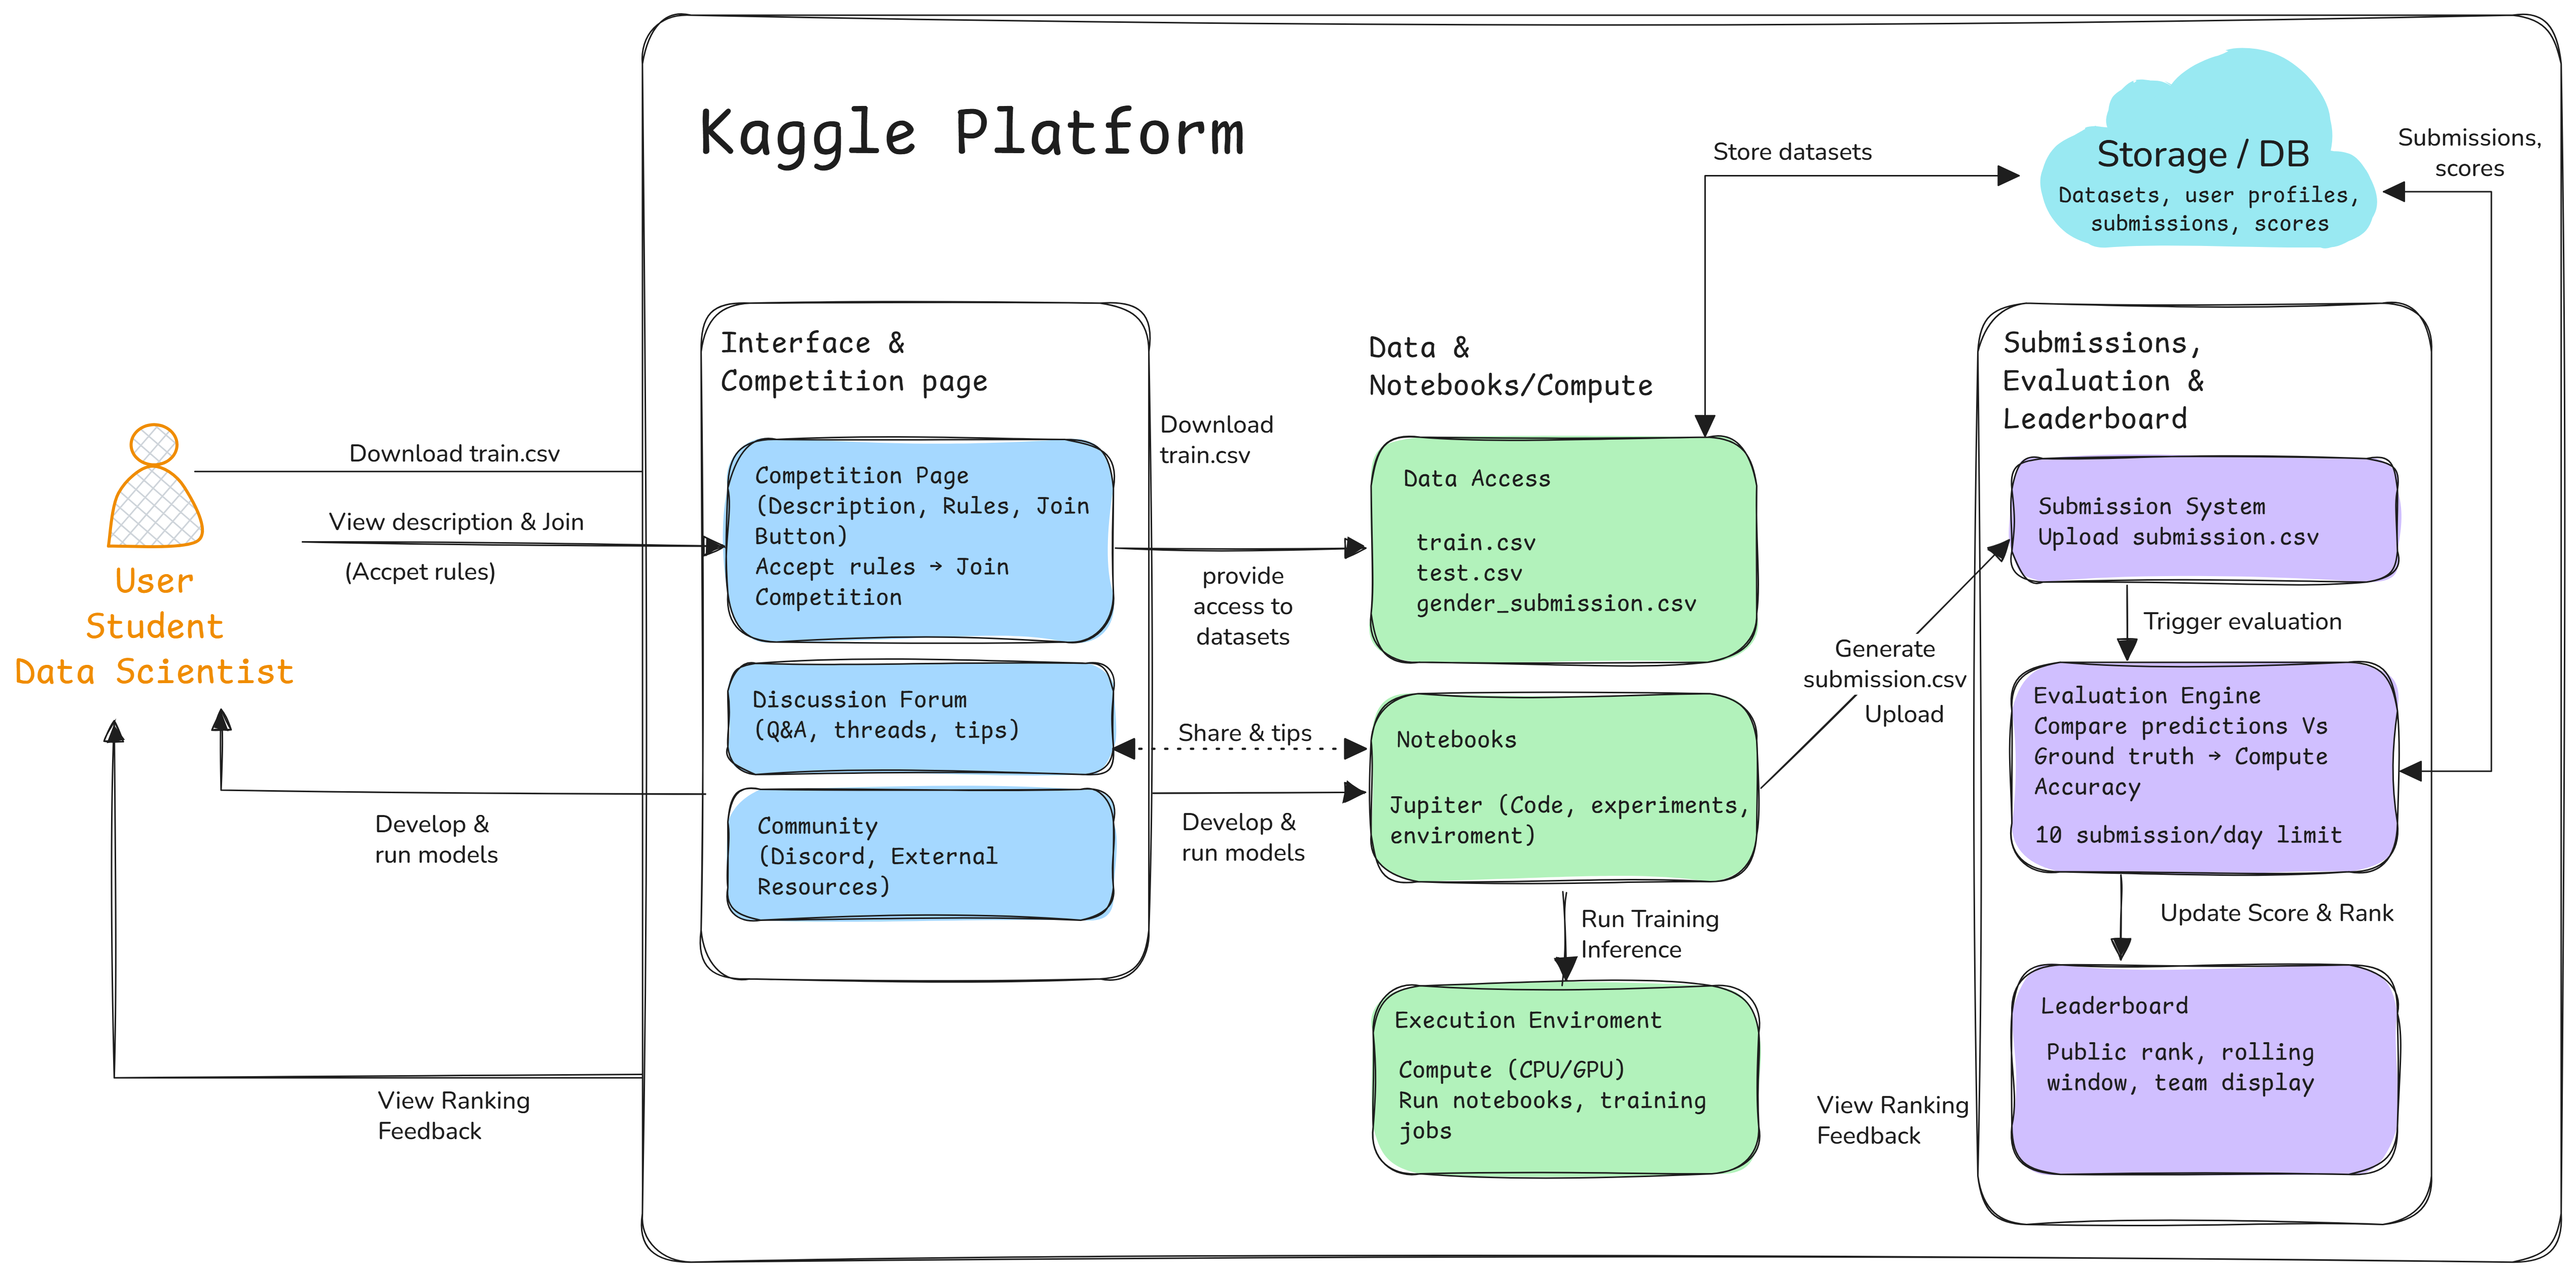
\includegraphics[width=\linewidth]{Figure1.png}
    \caption{Figure 1 shows the architecture of the Kaggle competition environment.}
    \label{fig:system-architecture}
\end{figure}

\noindent
\textbf{Figure \ref{fig:system-architecture}} shows the architecture of the Kaggle competition environment. 
The competitor accesses the Competition Page to join and download datasets (\texttt{train.csv}, \texttt{test.csv}). 
Model development occurs in Notebooks (Kaggle Notebooks), using Compute resources to train and produce \texttt{submission.csv}. 
The Submission System accepts submissions, and the Evaluation Engine computes the accuracy against the hidden ground truth, updating the public Leaderboard. 
Social and knowledge-sharing channels (Discussion Forum, Discord, GitHub) provide community feedback and starter code. 
Storage/DB centralizes datasets, user profiles, submissions and scores.

\end{document}
